% title: Shared and paired batch inputs
% description: Each box is a call to the same program. On the left panel, the two texts have a single prefix. On the right panel, each text has its own prefix. In both cases, each call produces a single output. The first entry of in_axes is for the text, and the second is for the prefix.
\documentclass[tikz,border=5pt]{standalone}
\usetikzlibrary{arrows.meta,calc,shapes.geometric}
\definecolor{numeric}{HTML}{4477AA}
\definecolor{textual}{HTML}{AA4499}

\tikzset{
    box/.style={draw, line width=0.8pt, minimum height=0.8cm,
                minimum width=1.8cm, inner sep=6pt, align=center},
    ir/.style={box},
    flow/.style={-{Stealth[length=5pt]}, line width=0.9pt},
    feedback/.style={flow, dashed},
    note/.style={font=\small, align=center},
    choice/.style={diamond, draw, line width=0.8pt,
                   aspect=2, inner sep=2pt, align=center},
}

\newcommand{\irframe}[2]{
    \draw[line width=0.8pt] #1 rectangle #2;
}

\newcommand{\transformarrow}[4][above]{
    \draw[flow] (#2) -- node[#1=6pt,note] {#4} (#3);
}


\tikzset{
    transform panel/.style={font=\small},
    transform program/.style={ir, minimum width=2.8cm},
}

\newcommand{\transformcanvas}{
    \path[use as bounding box] (-6.6,-2.75) rectangle (6.6,2.65);
}

\begin{document}
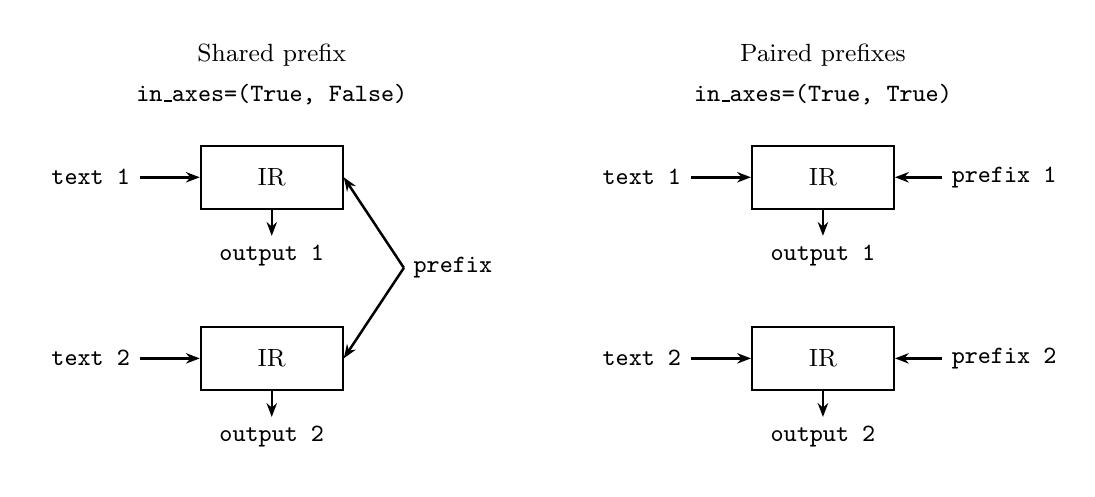
\begin{tikzpicture}[transform panel]
    \path[use as bounding box] (-6.6,-2.85) rectangle (6.6,2.75);

    \node at (-3.5,2.4) {Shared prefix};
    \node at (-3.5,1.9) {\texttt{in\_axes=(True, False)}};
    \node at (3.5,2.4) {Paired prefixes};
    \node at (3.5,1.9) {\texttt{in\_axes=(True, True)}};

    \node (prefix) at (-1.2,-0.3) {\texttt{prefix}};
    \foreach \i/\y in {1/0.85,2/-1.45} {
        \node (text\i) at (-5.8,\y) {\texttt{text \i}};
        \node[ir] (call\i) at (-3.5,\y) {IR};
        \node (output\i) at (-3.5,\y-1) {\texttt{output \i}};
        \draw[flow] (text\i.east) -- (call\i.west);
        \draw[flow] (prefix.west) -- (call\i.east);
        \draw[flow] (call\i.south) -- (output\i.north);

        \node (pairedtext\i) at (1.2,\y) {\texttt{text \i}};
        \node[ir] (pairedcall\i) at (3.5,\y) {IR};
        \node (pairedprefix\i) at (5.8,\y) {\texttt{prefix \i}};
        \node (pairedoutput\i) at (3.5,\y-1) {\texttt{output \i}};
        \draw[flow] (pairedtext\i.east) -- (pairedcall\i.west);
        \draw[flow] (pairedprefix\i.west) -- (pairedcall\i.east);
        \draw[flow] (pairedcall\i.south) -- (pairedoutput\i.north);
    }
\end{tikzpicture}
\end{document}
